\documentclass[a4paper]{article}
\usepackage[pdftex]{graphicx}
\usepackage[utf8]{inputenc}
\usepackage{enumerate}
\usepackage{siunitx}
\usepackage{colortbl}
\usepackage{tikz}
\usepackage{href-ul}
\hypersetup{
	colorlinks=true,
	linkcolor=blue,
	urlcolor=blue}
\sisetup{locale=DE}
\usepackage{icomma}
\usepackage{amssymb}
\usepackage{geometry}
\geometry{a4paper, top=15mm, left=15mm, right=15mm, bottom=15mm,
	headsep=10mm, footskip=12mm}

\begin{document}
	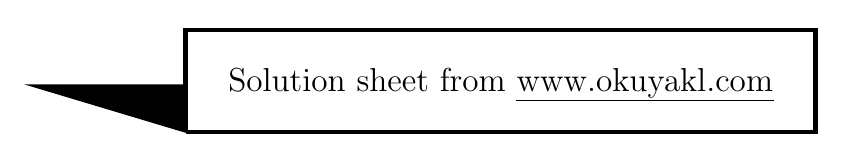
\begin{tikzpicture}(10,3)
		\draw[ultra thick](2,0) --(10,0) -- (10,1.3) --(2,1.3) -- (2,0);
		\draw[fill=black](2,0)-- (0,.6) -- (2,.6) -- (2,0);
		\node at (6,.6) {\large Solution sheet from \href{http://www.okuyakl.com}{www.okuyakl.com}};
	\end{tikzpicture}
	\vspace{0.5 cm}
	
	\noindent{\bf Task 1.}
	
	\renewcommand{\arraystretch}{2}
	\begin{tabular}{|>{\columncolor[gray]{.8}}p{3 cm}|p{3 cm}|p{3cm}|p{3 cm}|}
		\hline
		\rowcolor[gray]{.8} Body & Mass &Velocity & Kinetic Energy \\
		\hline
		Raindrops &$ \SI{0.05}{\gram} $&$ \SI{5}{\meter\per\second} $&$\SI{1.25}{\milli\joule}$\\
		\hline
		Table tennis ball &$ \SI{4.7}{\gram} $&$ \SI{10}{\meter\per\second} $&$\SI{0.47}{\joule}$ \\
		\hline
		Sprinter &$ \SI{75}{\kilo\gram} $&$ \SI{10}{\meter\per\second} $&$\SI{7.5}{\kilo\joule}$\\
		\hline
		Shooting star &$ \SI{0,1}{\gram} $&$ \SI{30}{\kilo\meter\per\second} $&$\SI{90}{\kilo\joule}$ \\
		\hline
		Football &$ \SI{0.42}{\kilo\gram} $&$ \SI{100}{\kilo\meter\per\hour} $&$\SI{324}{\joule}$ \\
		\hline
		Auto &$ \SI{1}{\tonne} $&$ \SI{130}{\kilo\meter\per\hour} $& $\SI{1.3}{\mega\joule}$ \\
		\hline
		Fighter jet &$ \SI{2}{\tonne} $&$ \SI{1200}{\kilo\meter\per\hour} $&$\SI{222}{\mega\joule}$\\
		\hline
		ICE &$ \SI{300}{\tonne} $&$ \SI{250}{\kilo\meter\per\hour} $&$\SI{1.4}{\giga\joule}$\\
		\hline
	\end{tabular}
	\vspace{1cm}
	
	\noindent{\bf Task 2. a)}
	The speed at points B and D is the same because the points are at the same height and no friction is calculated. To calculate the speed, we set the potential energy equal to the kinetic energy:
	$$
	\renewcommand{\arraystretch}{2}
	\begin{array}{rcll}
		W_{pot} &=& W_{kin}\\
		m\cdot g \cdot h &=& {1 \over 2} m v^2 &|:m\\
		g h &=& {1 \over 2} v^2 &| \cdot 2 \\
		2 g h &=& v^2 &| \sqrt{\quad}\\
		v &=& \sqrt{2 g h} &= \sqrt{2 \cdot \SI{9,81}{\meter\over{\second^2}} \cdot \SI{30}{\meter}}\\
		v &=& \SI{24}{\meter\per\second}
	\end{array}
	$$
	\vspace{0.5 cm}
	
	\noindent{\bf Task 2. b)}
	Mass is canceled out of the equation for calculating speed, so the speed would not change if the car were heavier.
	\vspace{0.5 cm}
	
	\noindent{\bf Task 2. c)}
	The braking energy is equal to braking force $F_B$ times distance $s$, the amount of energy is equal to the kinetic $W_{kin}$ and therefore equal to the potential $W_{pot}$:
	$$
	\renewcommand{\arraystretch}{2}
	\begin{array}{rcll}
		W_{pot}&=&F_B\cdot s & | :s\\
		F_B &=& {m g h \over s} &= {\SI{200}{\kilogram}\cdot \SI{9,81}{\meter\over{\second^2}} \cdot \SI{30}{\ meter}\over \SI{25}{\meter}}\\
		&=& \SI{2350}{\newton}
	\end{array}
	$$
	\vspace{0.5 cm}
	
	\newpage
	\noindent{\bf Task 3. a)}\\
	During free fall, positional energy=potential energy is converted into kinetic energy.
	The conservation of energy applies here:
	$$
	\renewcommand{\arraystretch}{2}
	\begin{array}{rcll}
		E_{kin} & = & E_{pot}\\
		{1 \over 2} \cdot m \cdot v^2 & = & m \cdot g \cdot h &| \cdot 2 \quad :m \\
		v^2 & = & 2\cdot g \cdot h & | \sqrt{\quad}\\
		v & = & \sqrt{ 2\cdot g \cdot h} \\
		v & = & \sqrt{ 2 \cdot \SI{9,81}{\meter\over{\second^2}}\cdot \SI{10}{\meter}} & = \SI{14}{\meter\ over\second}
	\end{array}
	$$
	\vspace{0.5 cm}
	
	\noindent{\bf Task 3. b)}\\
	We use the same approach but solve for height:
	$$
	\renewcommand{\arraystretch}{2}
	\begin{array}{rcll}
		E_{kin} & = & E_{pot}\\
		{1 \over 2} \cdot m \cdot v^2 & = & m \cdot g \cdot h &| :g \quad :m \\
		{v^2 \over 2 \cdot g} & = & h \\
		h & = &{(\SI{10}{\meter\over\second})^2 \over 2 \cdot \SI{9,81}{\meter\over{\second^2}}} & \approx \SI{5}{\meter}
	\end{array}
	$$
	\vspace{0.5 cm}
	
	\begin{center}
		\includegraphics[width=7 cm]{../../viecher/eendcomic.pdf}
		
		Here you can go back to the \href{https://www.okuyakl.de/phys/p8ekiL411/ae411.pdf}{task sheet}
	\end{center}
	
\end{document}